\documentclass[a4paper, 12pt]{article}

\usepackage{fontspec}
\usepackage[hidelinks]{hyperref}
\usepackage[catalan]{babel}
\usepackage{fullpage}
\usepackage{ragged2e}
\usepackage[a4paper, margin=2cm]{geometry}
\usepackage{graphicx}

\renewcommand*\contentsname{Índex}
\setlength\parindent{0pt}

\begin{document}
\title{Informe mecànic Projecte I}
\author{Marc Asenjo i Ponce de León \and
		Joan Marcè i Igual \and
		Iñigo Moreno i Caireta}
\date{\today}
\maketitle
\begin{center}
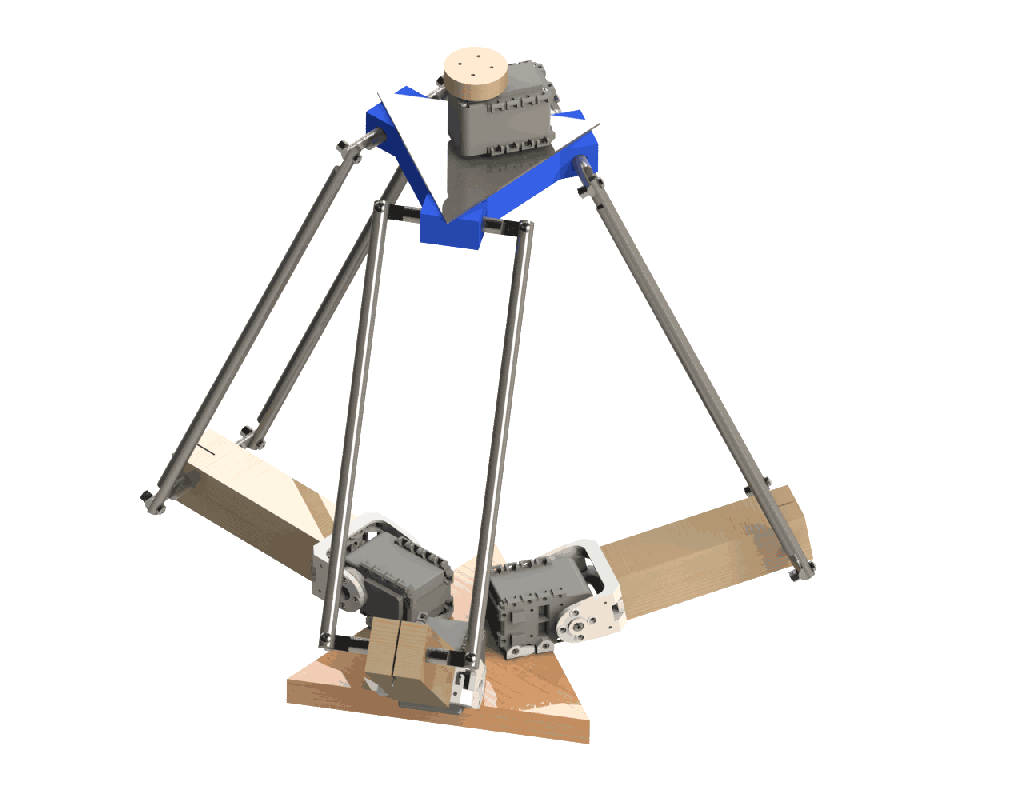
\includegraphics[width=0.4\textwidth]{./imgComp/logo}
\end{center}

\newpage
\tableofcontents{}

\newpage
\section{Objectiu}
El nostre objectiu és construir un robot delta que sigui capaç de posicionar peces de dominó de la manera desitjada per l'usuari, aquest tindrà un programa que li permetrà dibuixar el circuit desitjat i també podrà controlar el robot mitjançant un joystick.

\newpage
\section{Informe mecànic}
\section{Informe mecànic}
\subsection{Assemblatge general}

Aquest robot delta està format per quatre parts generals: els servos, els braços, els avantbraços i la pinça final. 

El robot consta de tres servos que permetran el posicionament de la pinça; cada servomotor té acoblat un braç que es mou junt amb l'eix d'aquest. A més a més, els
braços estan units mitjançant un eix amb l'avantbraç. Tots els avantbraços arriben a unir-se a la peça final que és la pinça permetent així que el moviment dels tres servos determini un punt a l'espai en el qual posicionar la pinça amb tres graus de llibertat de translació.

\begin{figure}[h!]
\centering
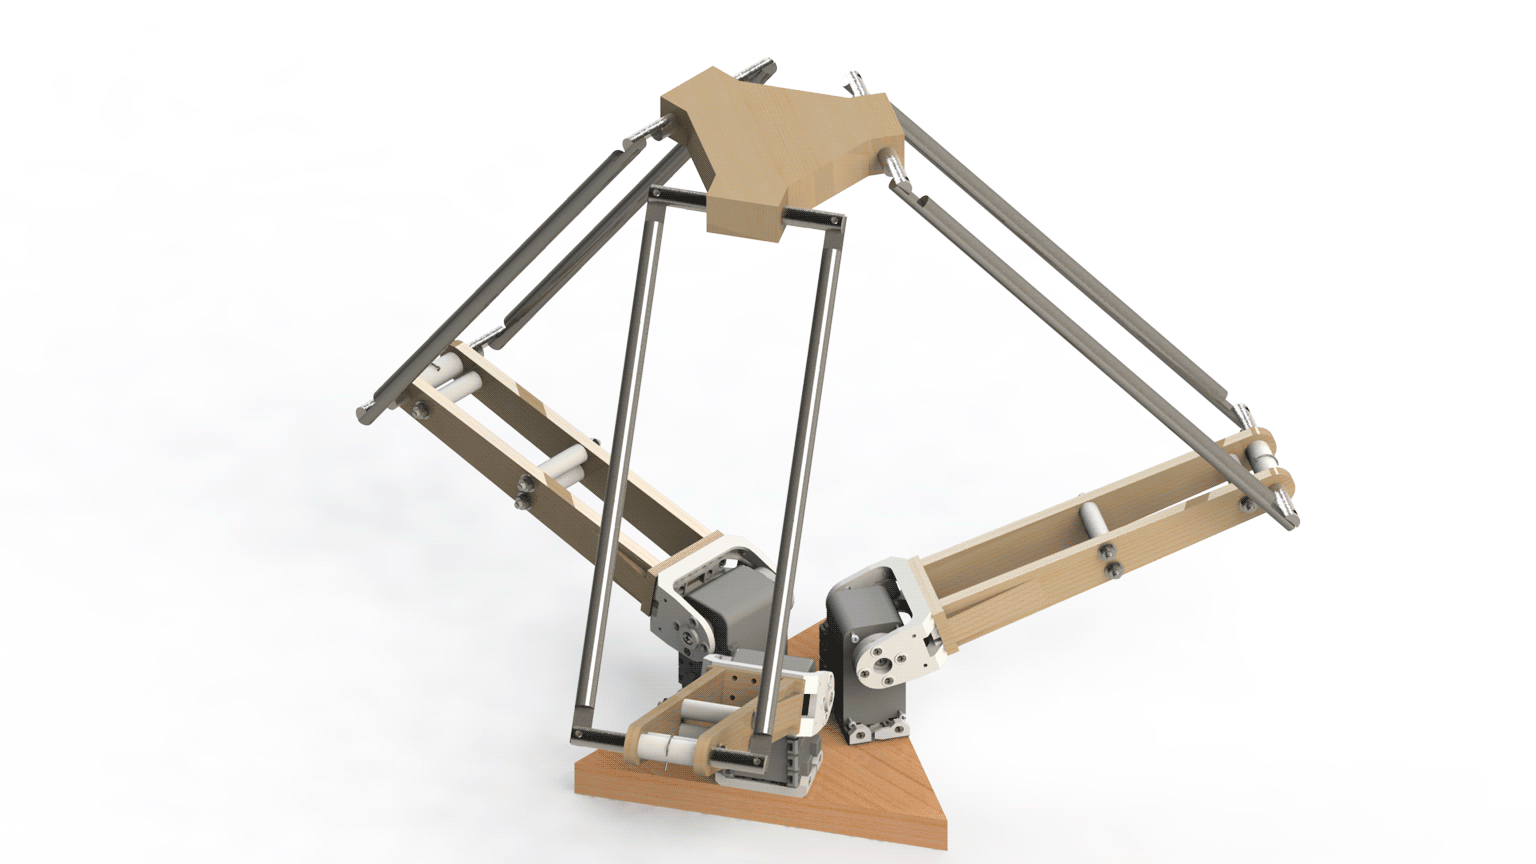
\includegraphics[width=10cm]{./imgComp/general}
\caption{Assemblatge general}
\end{figure}



\newpage
\subsection{Servomotors}
Els servomotors permeten el posicionament específic d'un eix a un cert angle. N'hi ha tres. S'utilitza el model AX-12 de dynamixel. 

A part dels servos també s'han utilitzat els accessoris \emph{FP04-F2 i FP04-F3}. Per tal de facilitar l'ancoratge entre el servomotor i les diferents peces.

\begin{figure}[h!]
\centering
\begin{minipage}[b]{0.45\linewidth}
\centering
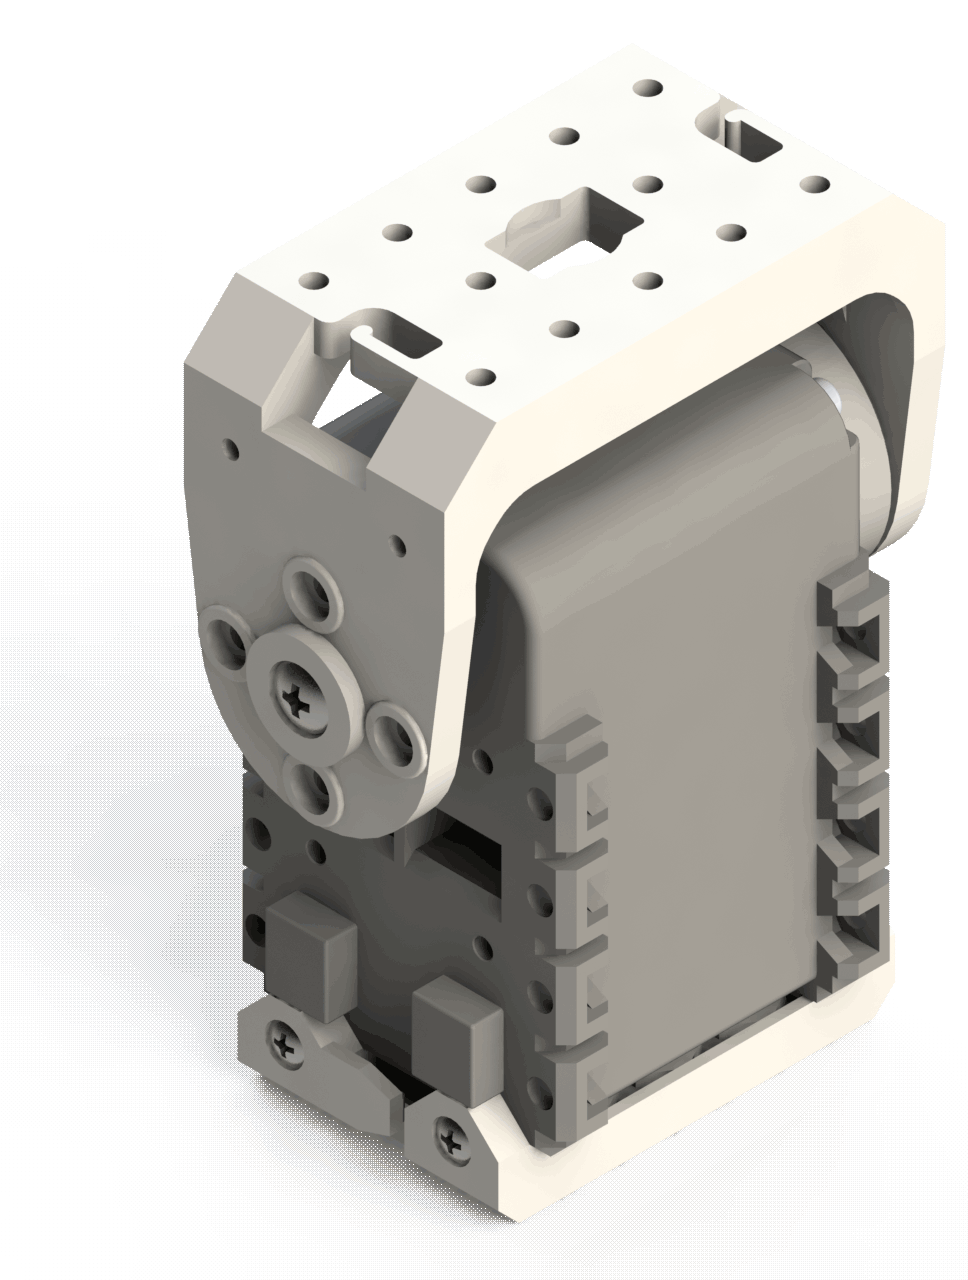
\includegraphics[width=6cm]{./imgComp/servo}
\caption{Imatge 3D del servomotor}
\end{minipage}
\begin{minipage}[b]{0.45\linewidth}
\centering
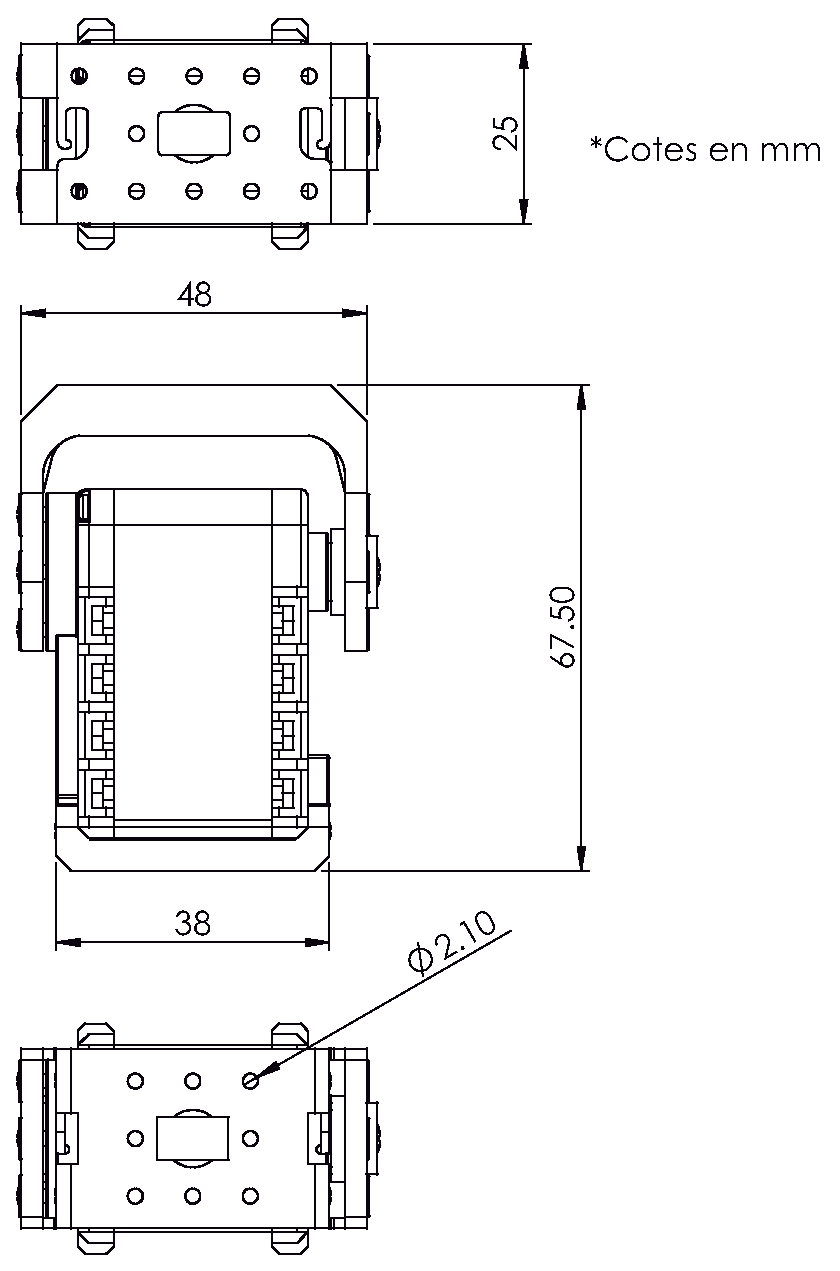
\includegraphics[width=7cm]{./sketch/servo}
\caption{Plànol servo amb accessoris}
\end{minipage}
\end{figure}

\subsubsection{Plataforma suport}
Sobre aquesta plataforma estaran situats els tres servos del robot. Serà de fusta ja que permetrà cargolar els servomotors a sobre i així impedir un moviment no desitjat.
\begin{figure}[h!]
\centering
\begin{minipage}[b]{0.45\linewidth}
\centering
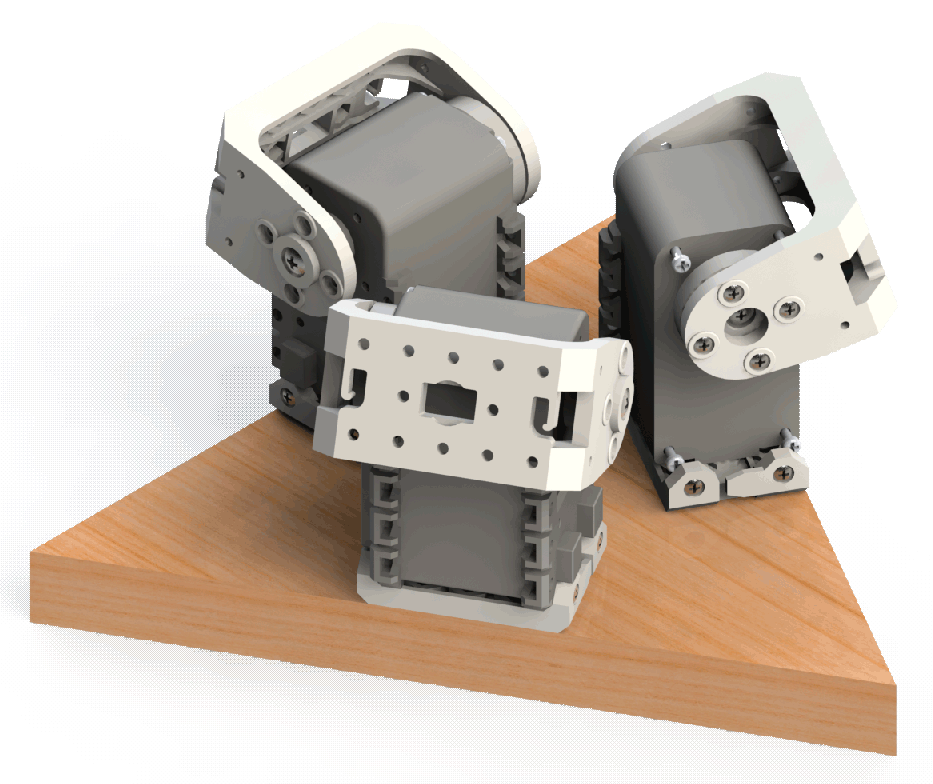
\includegraphics[width=6cm]{./imgComp/plataforma}
\caption{Plataforma amb els servos posats}
\end{minipage}
\hfill
\begin{minipage}[b]{0.45\linewidth}
\centering
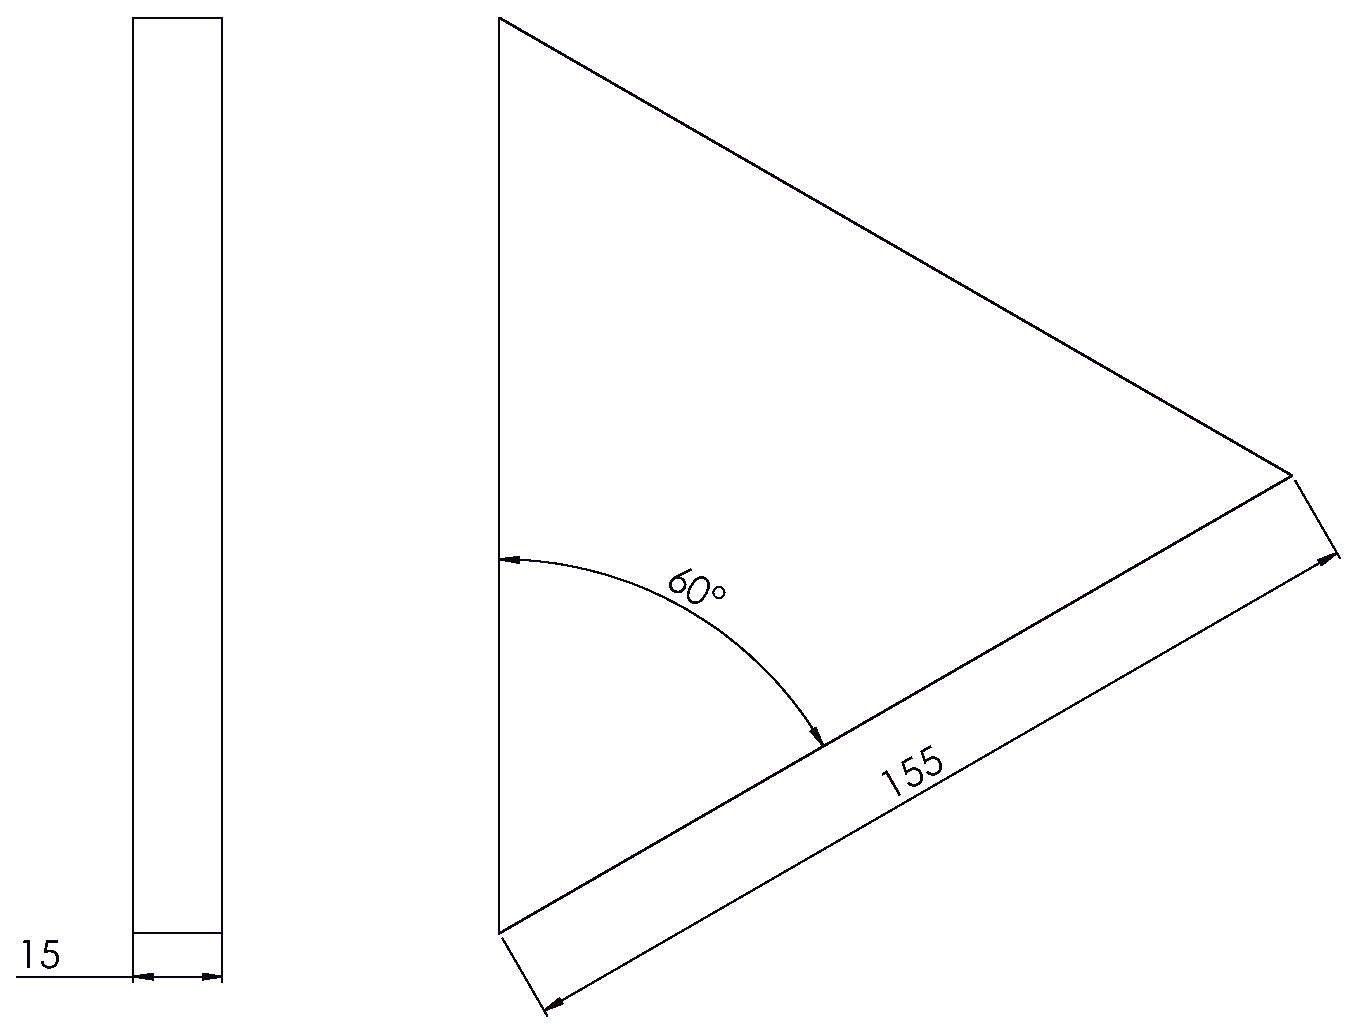
\includegraphics[width=7cm]{./sketch/plataforma}
\caption{Plànol plataforma servos}
\end{minipage}
\end{figure}


%------------
% BRAÇ
%------------
\newpage
\subsection{Braç - inicial}
Es recolza en els servomotors i principalment està fet de fusta. La part estructural és tota de fusta i està tota enganxada amb cola i després hi ha tres estabilitzadors que eviten vibracions innecessàries a la part del braç més propera a l'eix. 

\begin{figure}[h!]
\begin{minipage}[b]{0.45\linewidth}
\centering
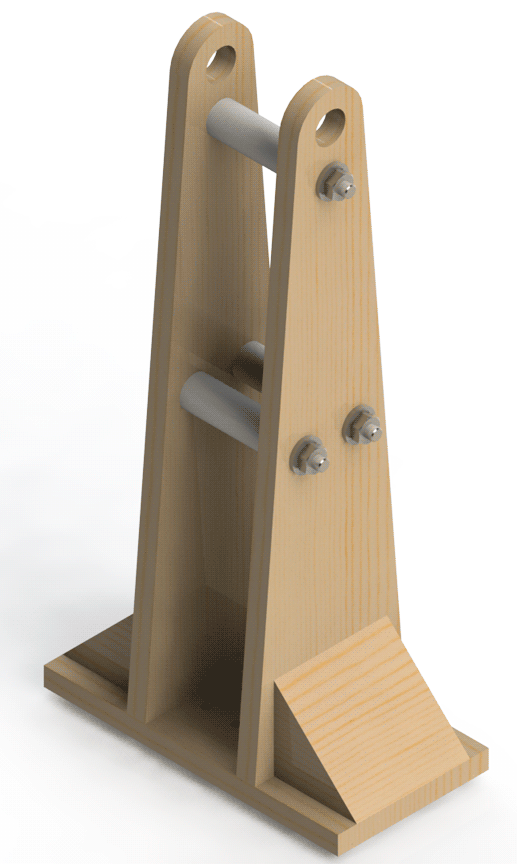
\includegraphics[height=8cm]{./imgComp/brac}
\caption{Braç muntat}
\end{minipage}
\begin{minipage}[b]{0.45\linewidth}
\centering
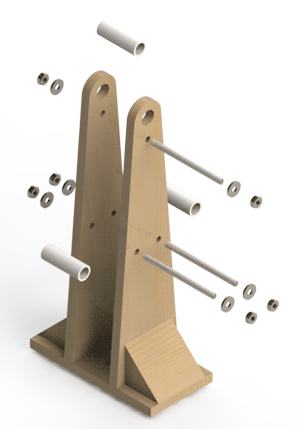
\includegraphics[height=8cm]{./imgComp/brac_expl}
\caption{Muntatge del braç}
\end{minipage}
\end{figure}

\subsubsection{Estructura}
L'estructura està feta amb llistons de fusta. S'ha utilitzat un llistó de 45º d'inclinació per la part de suport que es troba entre la base i la columna vertical i per a fer tant la base com les columnes verticals s'ha utilitzat un llistó de 5 mm de gruix que s'ha tallat perquè tingui la forma desitjada. 

La raó per la que s'ha escollit fer-ho amb fusta és per poder fer-hi forats i talls amb relativa facilitat ja que la fusta és fàcil de treballar; també el reduït cost econòmic d'aquesta ha motivat escollir aquest material.
\begin{figure}[h!]
\begin{minipage}[b]{.45\linewidth}
\centering
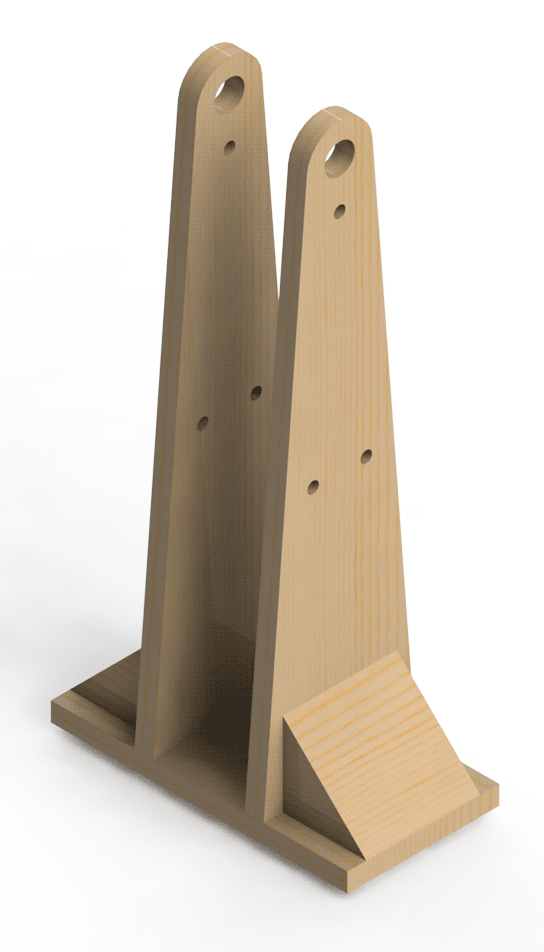
\includegraphics[height=8cm]{./imgComp/estructura}
\caption{Estructura del braç}
\end{minipage}
\begin{minipage}[b]{.45\linewidth}
\centering
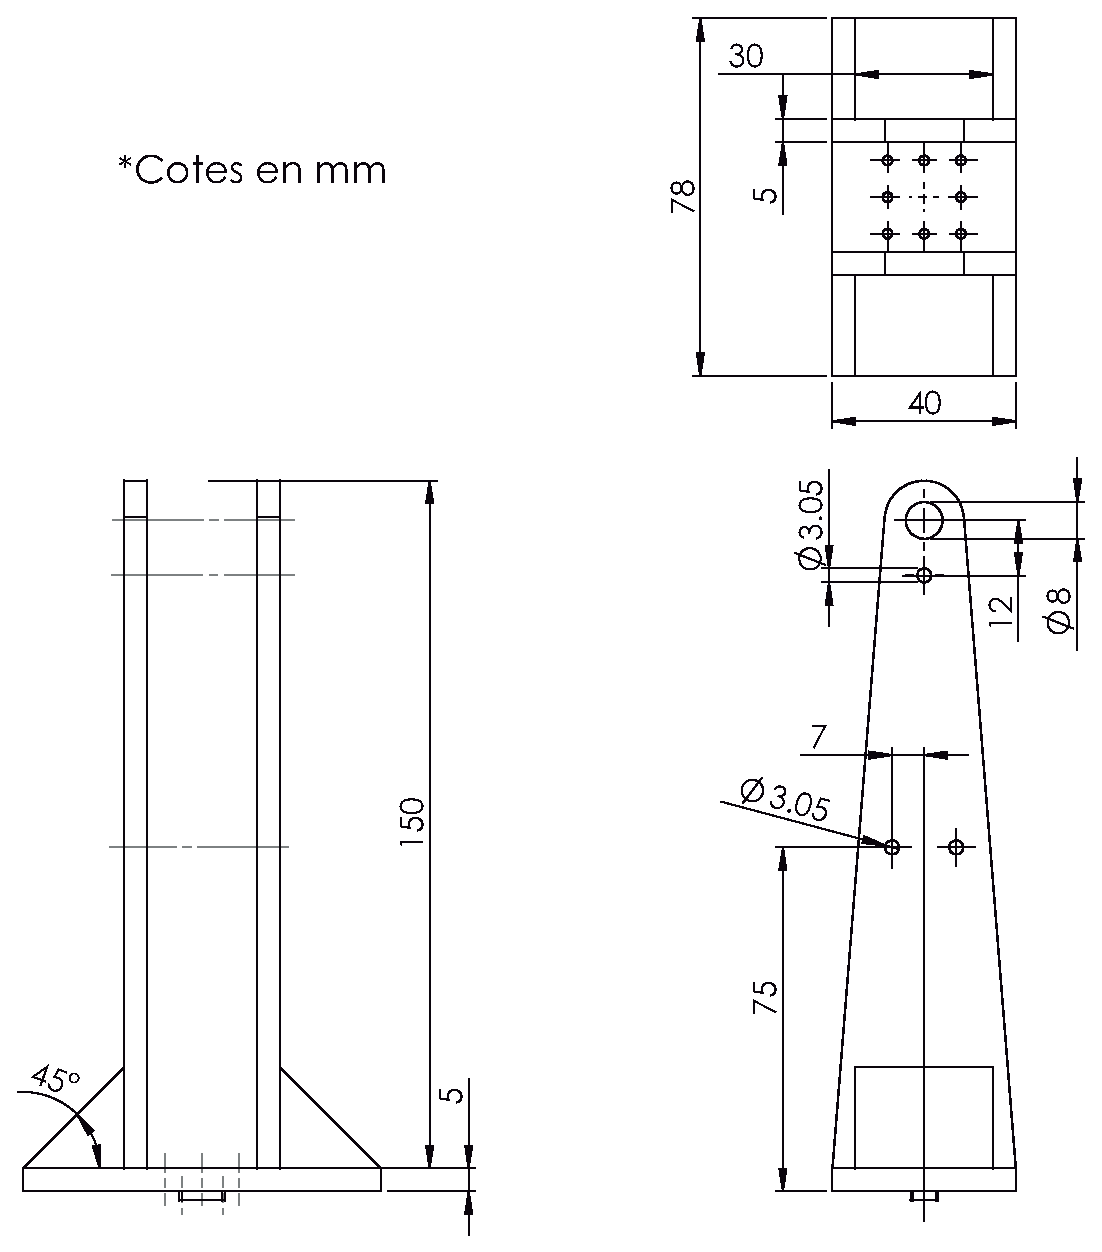
\includegraphics[height=10cm]{./sketch/estructura}
\caption{Plànol de les mides del braç}
\end{minipage}
\end{figure}

\subsubsection{Estabilitzador}
L'estabilitzador s'utilitza per tal que l'estructura de fusta no vibri ni es deformi degut al moviment del robot. 
És un conjunt de peces que està format per:
\begin{itemize}
\item Una barra roscada de M3 i 45 mm de llargada

\item Un tub de plàstic de 6 mm de diàmetre interior i 8 mm de diàmetre exterior de 24 mm de llargada

\item Dues volanderes

\item Dues femelles M3
\end{itemize}

El tub de plàstic es situa entre les dues fustes verticals de l'estructura del braç i per dins hi va la barra roscada. A fora es col·loquen les femelles i les volanderes de manera que permeten prémer les dues fustes contra el tub de plàstic forçant així que la distància entre les dues fustes sigui constant.

\begin{figure}[h!]
\begin{minipage}[b]{0.45\linewidth}
\centering
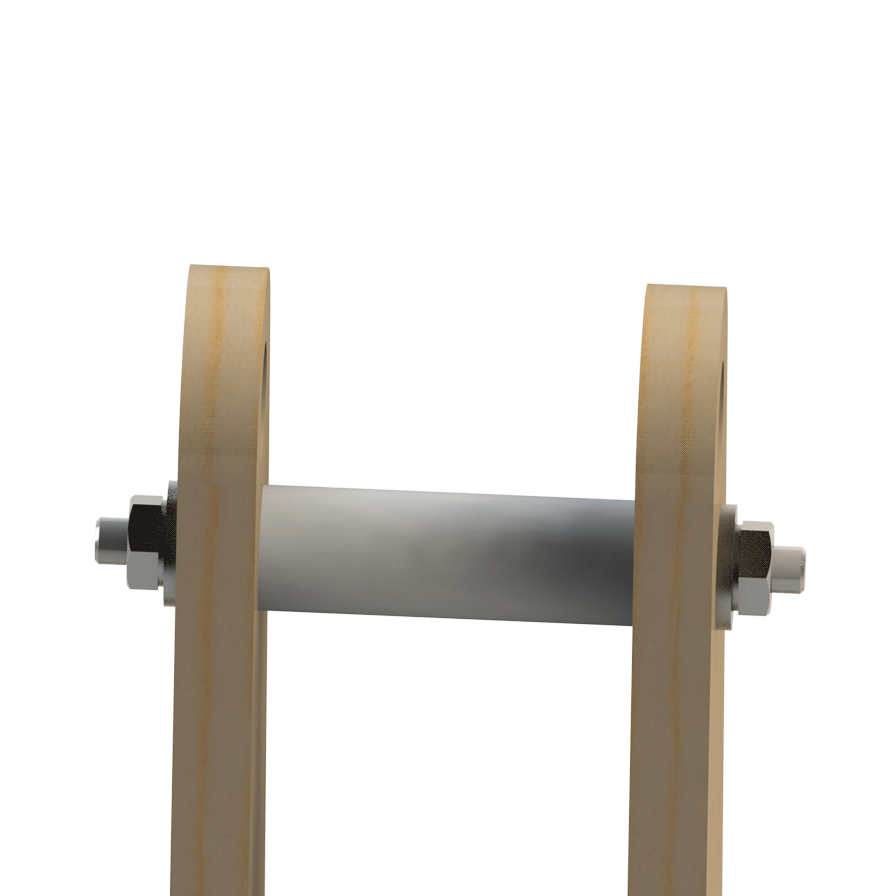
\includegraphics[height=5cm]{./imgComp/estab}
\caption{Estabilitzador muntat}
\end{minipage}
\begin{minipage}[b]{0.45\linewidth}
\centering
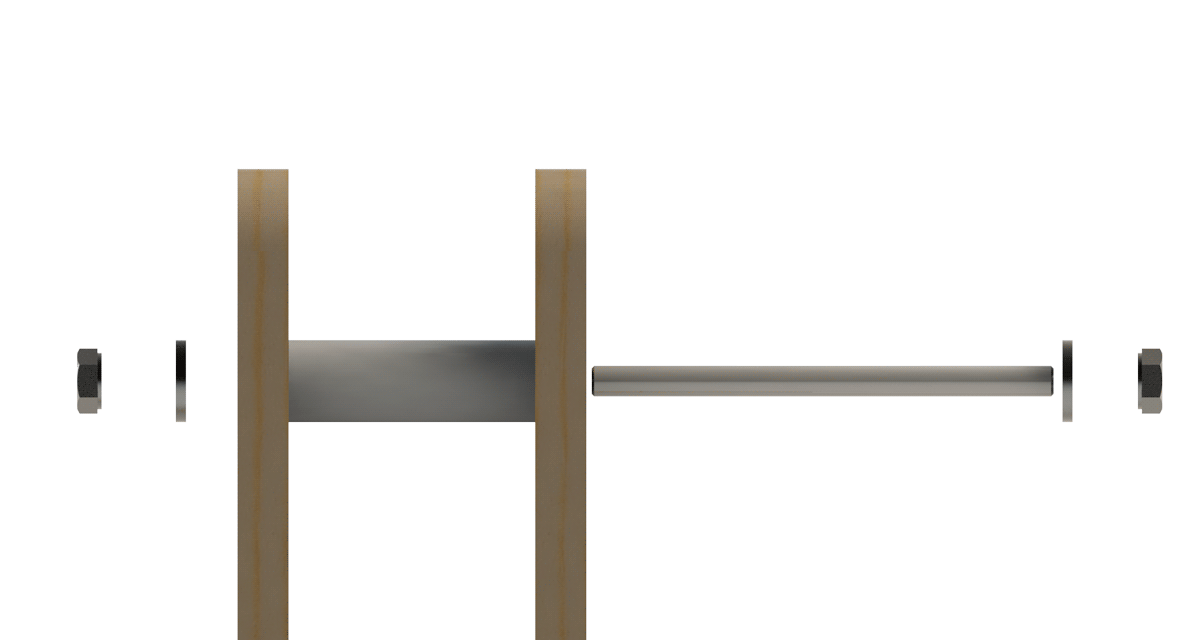
\includegraphics[height=5cm]{./imgComp/estab_expl}
\caption{Muntatge estabilitzador}
\end{minipage}
\end{figure}

\subsection{Braç - final}
El braç inicial era massa llarg així que es va haver de fer un nou model més curt, el nou model és més senzill ja que es va veure que un model massa elaborat era difícil de construir correctament i amb les mides especificades. 

\begin{figure}[h!]
\hfill
\begin{minipage}{0.45\linewidth}
\centering
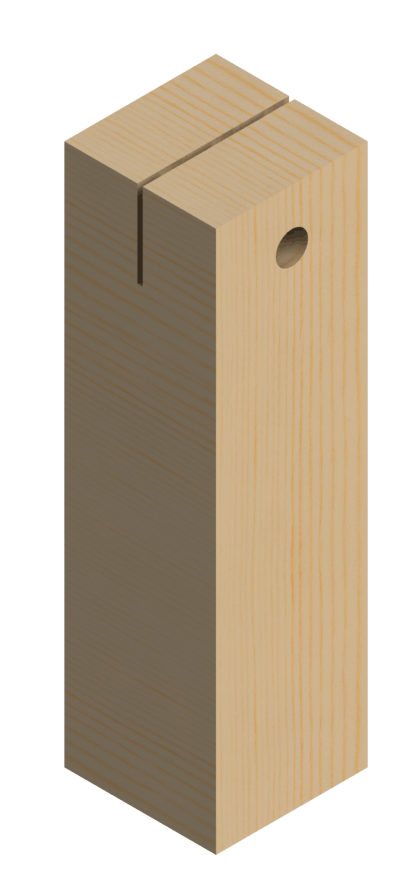
\includegraphics[height=7cm]{./imgComp/brac_nou}
\caption{Nou braç}
\end{minipage}
\hfill
\begin{minipage}{0.45\linewidth}
\centering
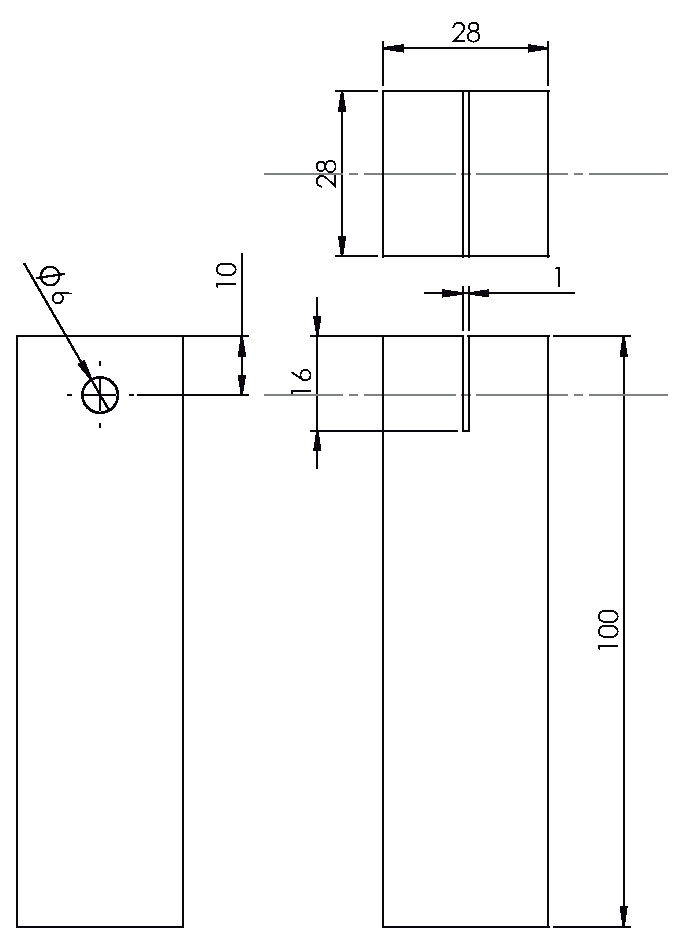
\includegraphics[height=7cm]{./sketch/brac_nou}
\caption{Nou braç}
\end{minipage}
\hfill
\end{figure}

%---------------
% AVANTBRAÇ
%---------------
\newpage
\subsection{Avantbraç}
L'avantbraç ha de connectar el braç amb la pinça i ha d'estar fet de tal manera que les dues rectes que hi ha entre els eixos sempre siguin paral·leles, a part la unió amb el braç i la pinça ha de ser mitjançant una junta esfèrica. En aquest robot s'ha separat la junta esfèrica en dos eixos per tal que faci la mateixa funció i sigui més fàcil de fabricar.

\begin{figure}[h!]
\begin{minipage}[b]{.45\linewidth}
\centering
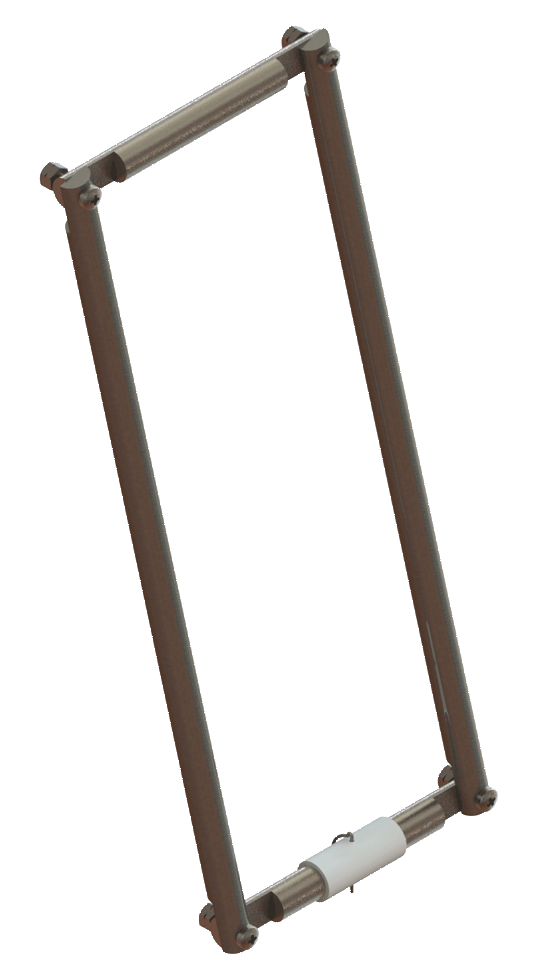
\includegraphics[height=7cm]{./imgComp/avant}
\caption{Avantbraç muntat}
\end{minipage}
\begin{minipage}[b]{.45\linewidth}
\centering
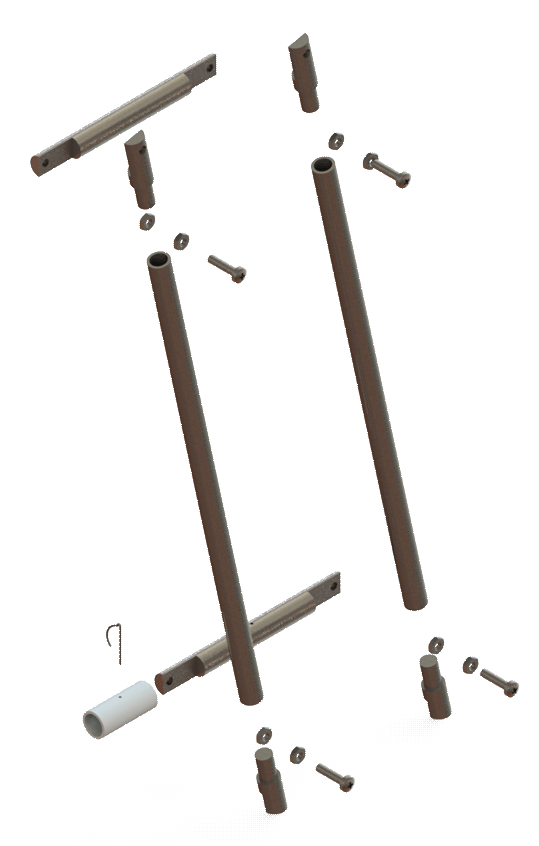
\includegraphics[height=7cm]{./imgComp/avant_expl}
\caption{Muntatge avantbraç}
\end{minipage}
\end{figure}

\subsubsection{Vara unió}
És la que uneix l'eix situat a la pinça i l'eix situat al braç. És d'alumini que és un metall bastant lleuger i, a més a més, s'ha pensat en fer-la buida per dins per tal d'estalviar pes i així evitar errors en el posicionament final del robot.
\begin{figure}[h!]
\centering
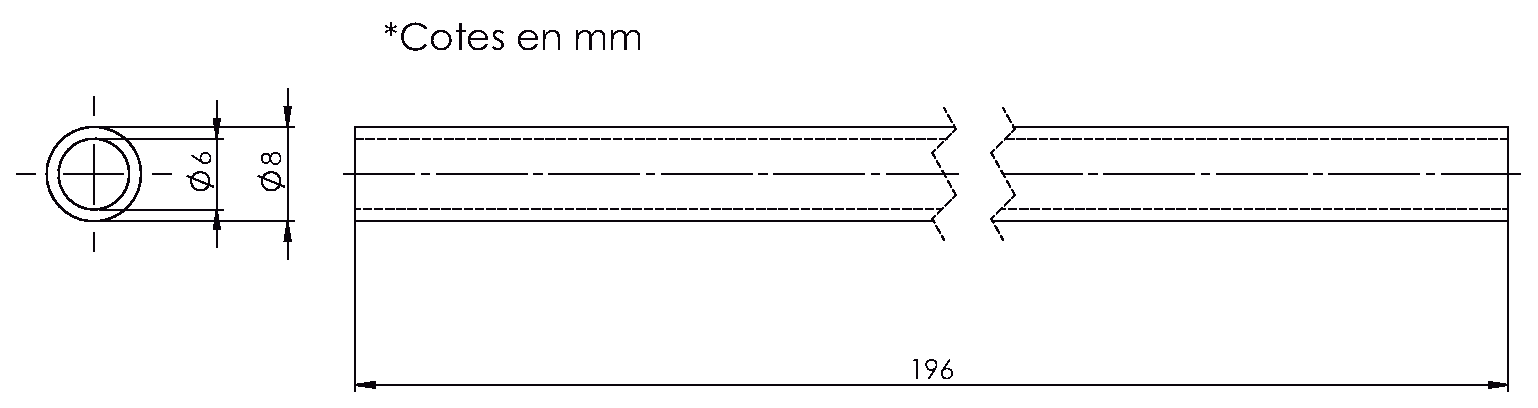
\includegraphics[width=15cm]{./sketch/vara}
\caption{Plànol de la vara}
\end{figure}

\subsubsection{Eix Braç}
És el que es troba situat al braç de cada servo, el material utilitzat també ha estat l'alumini ja que és un material prou resistent com per fer d'eix i a la vegada també és fàcil de perforar.
Aquest eix té un petit forat just al mig per tal de poder posar-hi un passador i que així quedin units l'eix i un tub de plàstic que estarà situat entre les dues columnes del braç; d'aquesta manera s'espera que l'eix es mantingui centrat i lateralment. El tub de plàstic tindrà les mateixes mides que la separació entre les columnes.
\begin{figure}[h!]
\centering
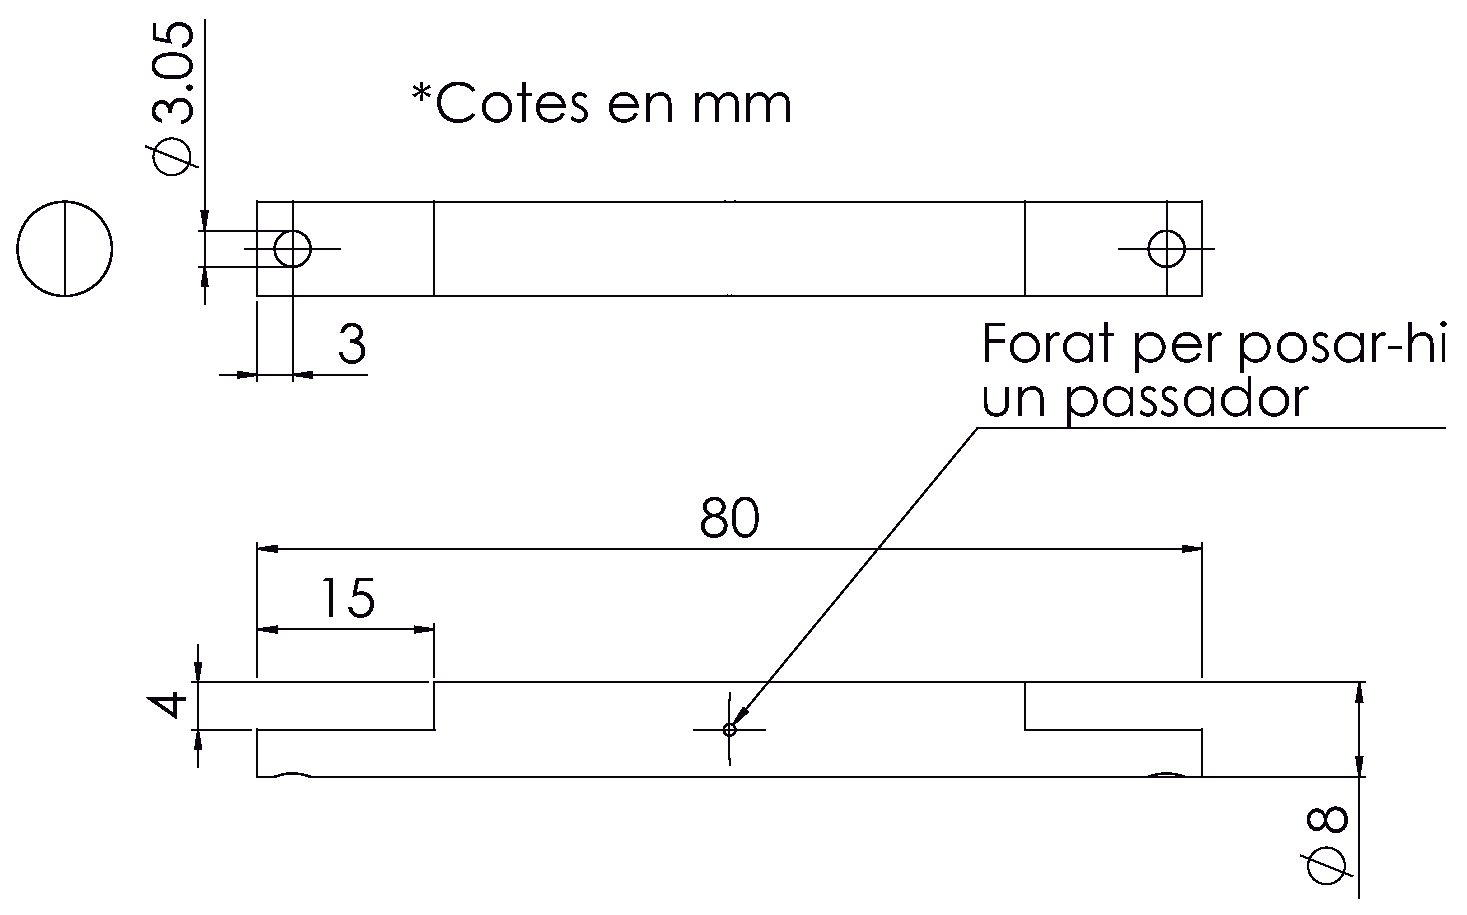
\includegraphics[width=8cm]{./sketch/eix}
\caption{Plànol de l'eix}
\end{figure}

\subsubsection{Eix Pinça}
És l'eix que estarà situat al suport de la pinça, és exactament igual a l'eix del braç a excepció que aquest no estarà centrat mitjançant un passador. Un cop muntat al suport de la pinça, hi haurà una goma a cada costat de l'eix del suport de la pinça per evitar el moviment lateral.
\begin{figure}[h!]
\centering
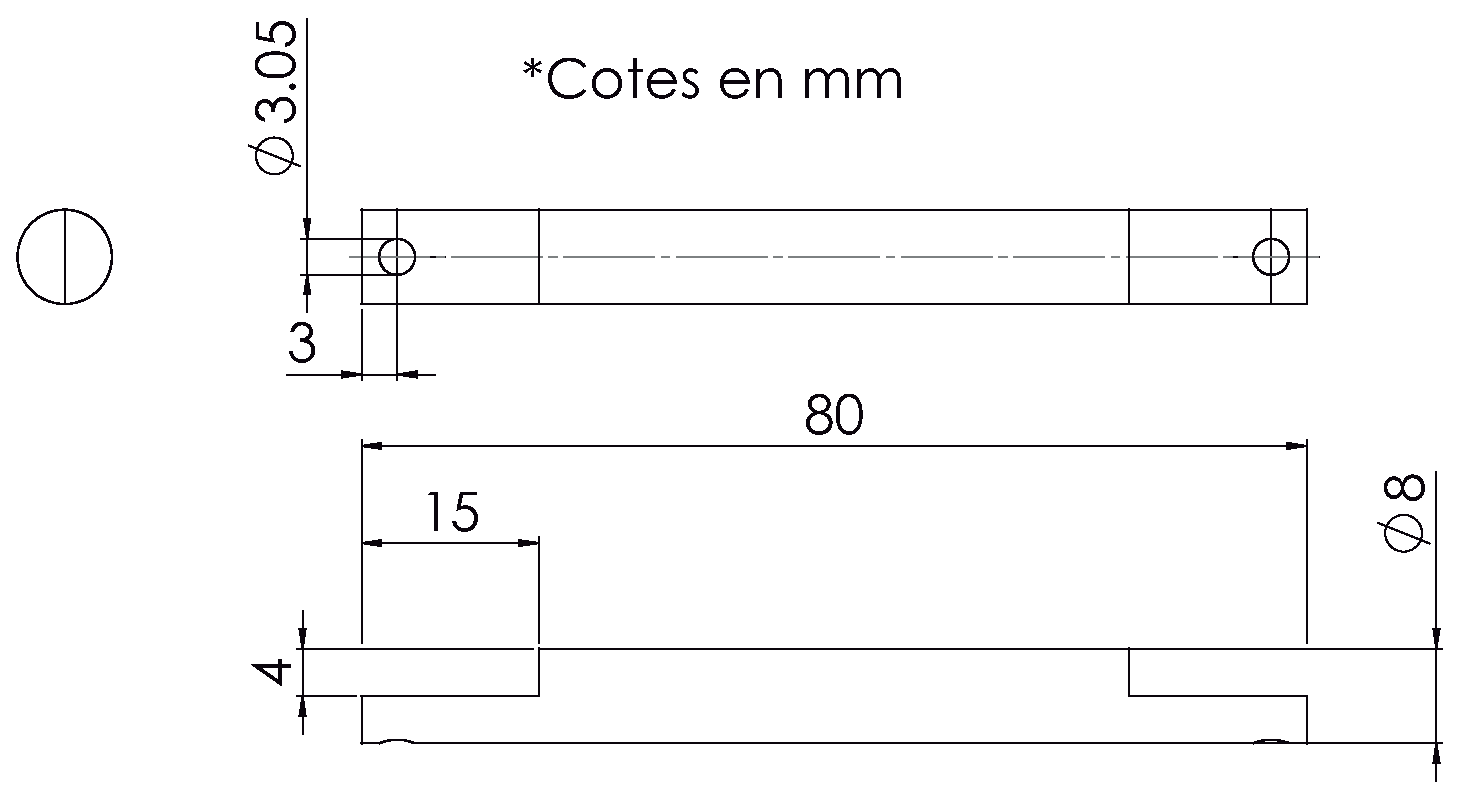
\includegraphics[width=8cm]{./sketch/eix2}
\caption{Plànol de l'eix de la pinça}
\end{figure}

\subsubsection{Unió}
Amb aquesta peça es pretén unir la vara a l'eix. Està feta de manera que la part que té un radi de 6 mm entri dins del forat interior de la vara i quedi fixat allà. D'aquesta manera s'acaba tenint el mateix resultat a tenir una sola vara amb els forats d'unió a cada costat però amb un pes inferior.
\begin{figure}[h!]
\centering
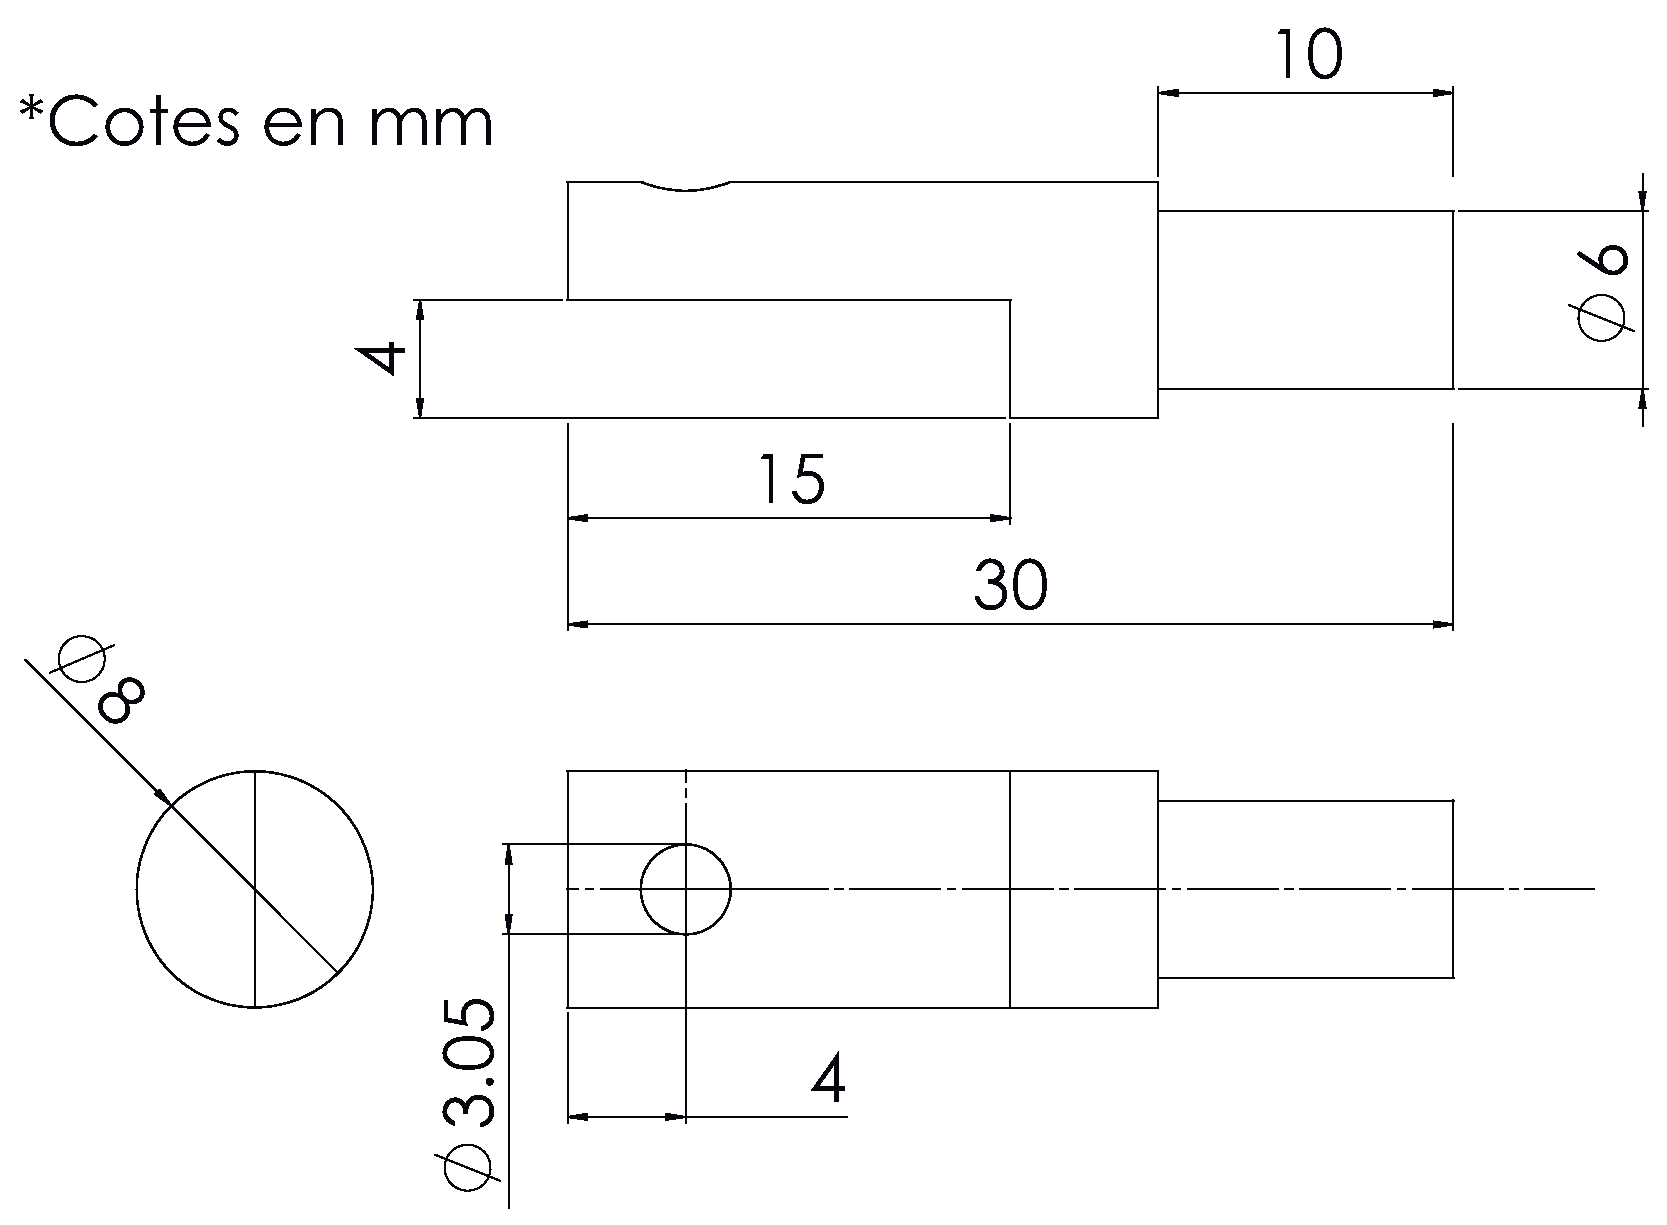
\includegraphics[width=8cm]{./sketch/unio}
\end{figure}


%--------
% PINÇA
%--------
\subsection{Pinça}
De moment només s'ha pensat el suport de la pinça ja que fins que no estigui aquesta part muntada i provat el seu correcte funcionament no es pot estar segur a seguir afegint més components. 
El suport serà de plàstic, imprès en 3D ja que la fusta aquí resulta ser un element massa dèbil i en el moment de fer els forats per on ha de passar l'eix, es trenca.
\begin{figure}[h!]
\centering
\begin{minipage}[b]{0.45\linewidth}
\centering
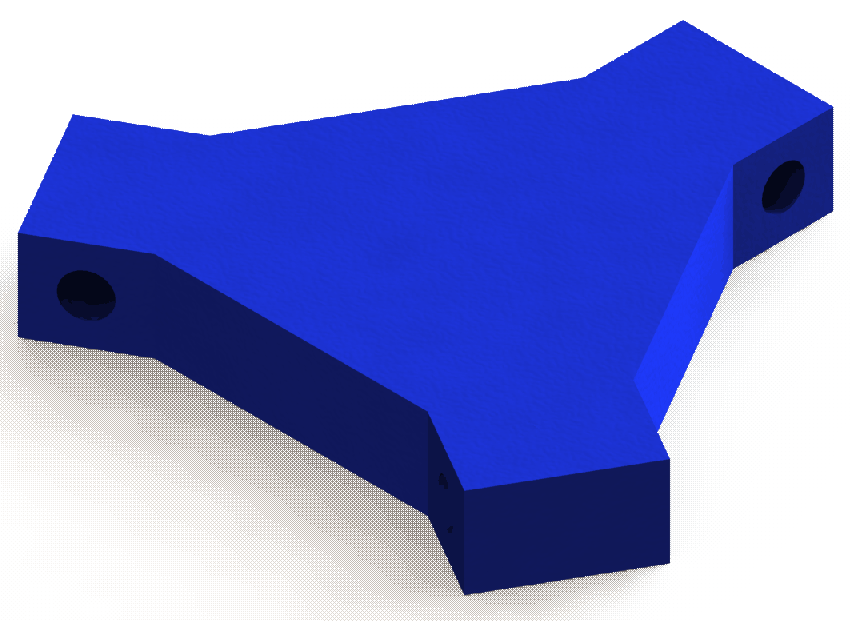
\includegraphics[width=8cm]{./imgComp/pinca}
\caption{Representació 3D del suport de la pinça}
\end{minipage}
\hfill
\begin{minipage}[b]{0.45\linewidth}
\centering
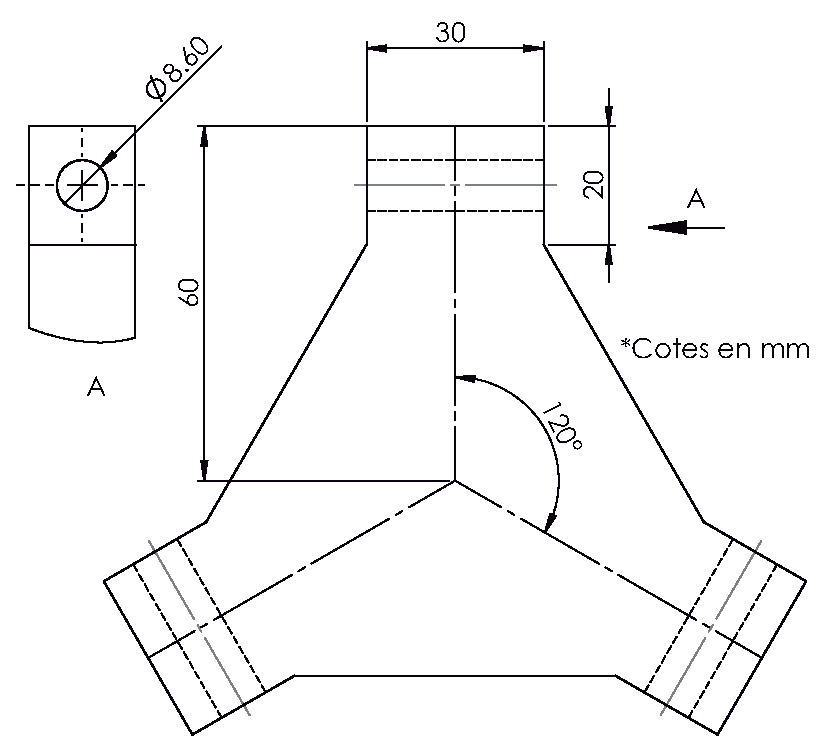
\includegraphics[width=9cm]{./sketch/pinca}
\caption{Plànol del suport de la pinça}
\end{minipage}
\end{figure}


\newpage
\section{Informe cinemàtic}
\section{Informe cinemàtic}
\subsection{Cinemàtica inversa}

El càlcul invers és el que serveix per trobar els angles a partir de la posició a la que es vol situar la plataforma. Es pot fer el càlcul per cada motor de manera separada. Primer s'han de definir les mides principals del robot que s'usaran en el càlcul.

\subsubsection{Definicions de variables}
\begin{figure}[h!]
\centering
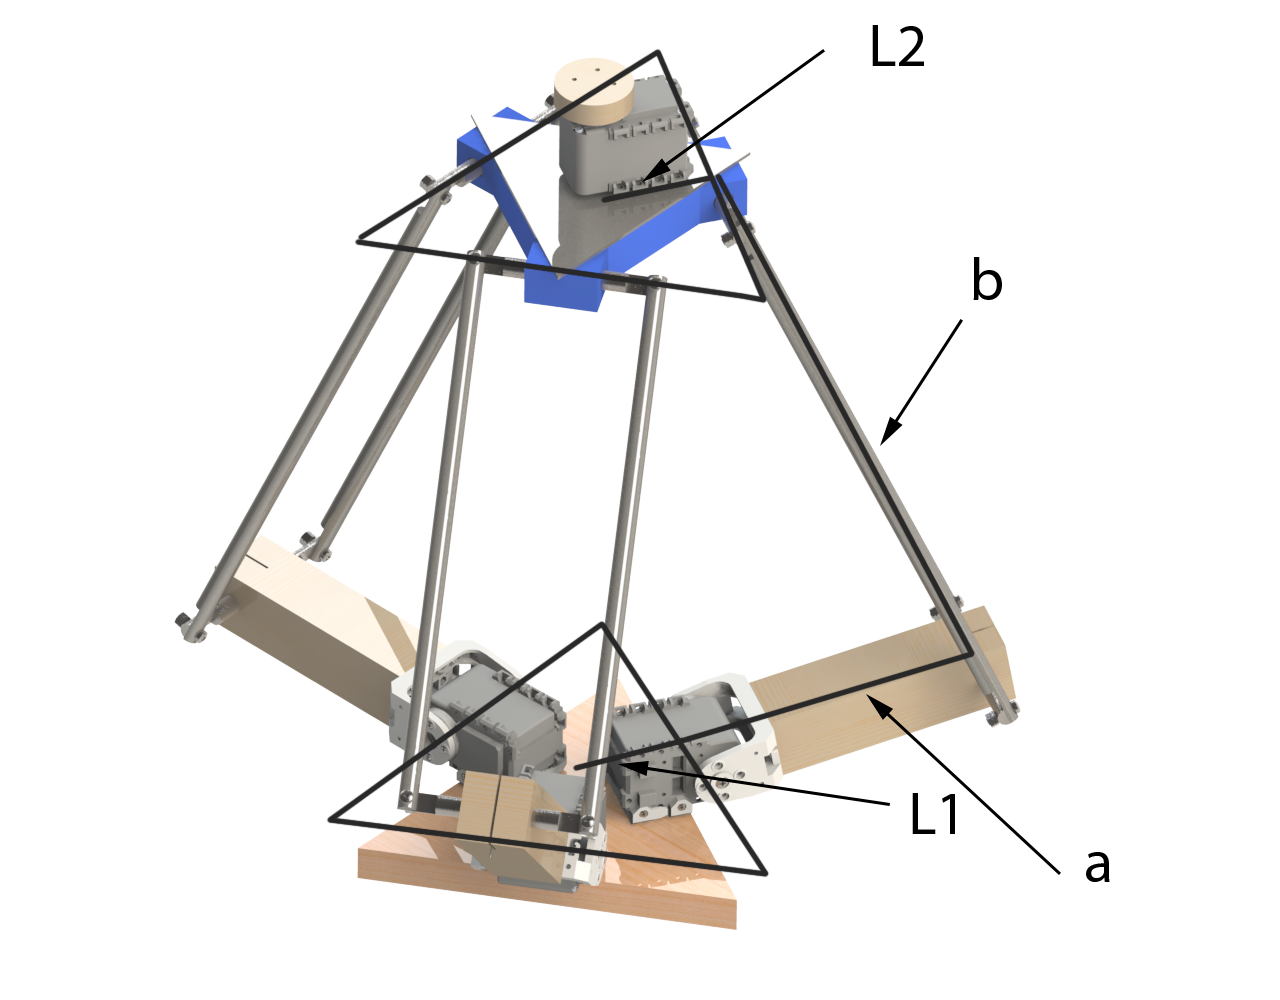
\includegraphics[width=12cm]{./imgComp/esquema_general}
\end{figure}

\begin{description}
\item[a] és la mida total del braç, des de l'eix del motor fins a l'eix de la connexió amb l'avantbraç.
\item[b] és la mida de tot l'avantbraç des de la connexió amb el braç fins a la unió amb la plataforma.
\item[L1] és la distància entre el centre de la base als eixos dels motors.
\item[L2] és la distància entre el centre de la plataforma a l'eix de connexió amb l'avantbraç.
\end{description}

\subsubsection{Canvis de base}
Com el càlcul de cada angle és independent de la resta, es poden fer canvis de base per poder fer-ho tot amb una sola funció a l'hora de programar. La base inicial $\{x_0,y_0,z_0\}$ està al centre de la base, amb la $x$ en la direcció del motor 1. Les bases $\{x_i,y_i,z_i\}$ que s'utilitzaran per calcular l'angle del motor $i$ estan posicionades al centre del eix de cada motor, i la seva $x$ apunta en la direcció perpendicular al eix del motor. També es suma $L2$ a $x_i$ per fer que la posició objectiu sigui el punt de connexió entre la plataforma i l'avantbraç en lloc del centre de la plataforma.

\begin{figure}[h!]
\centering
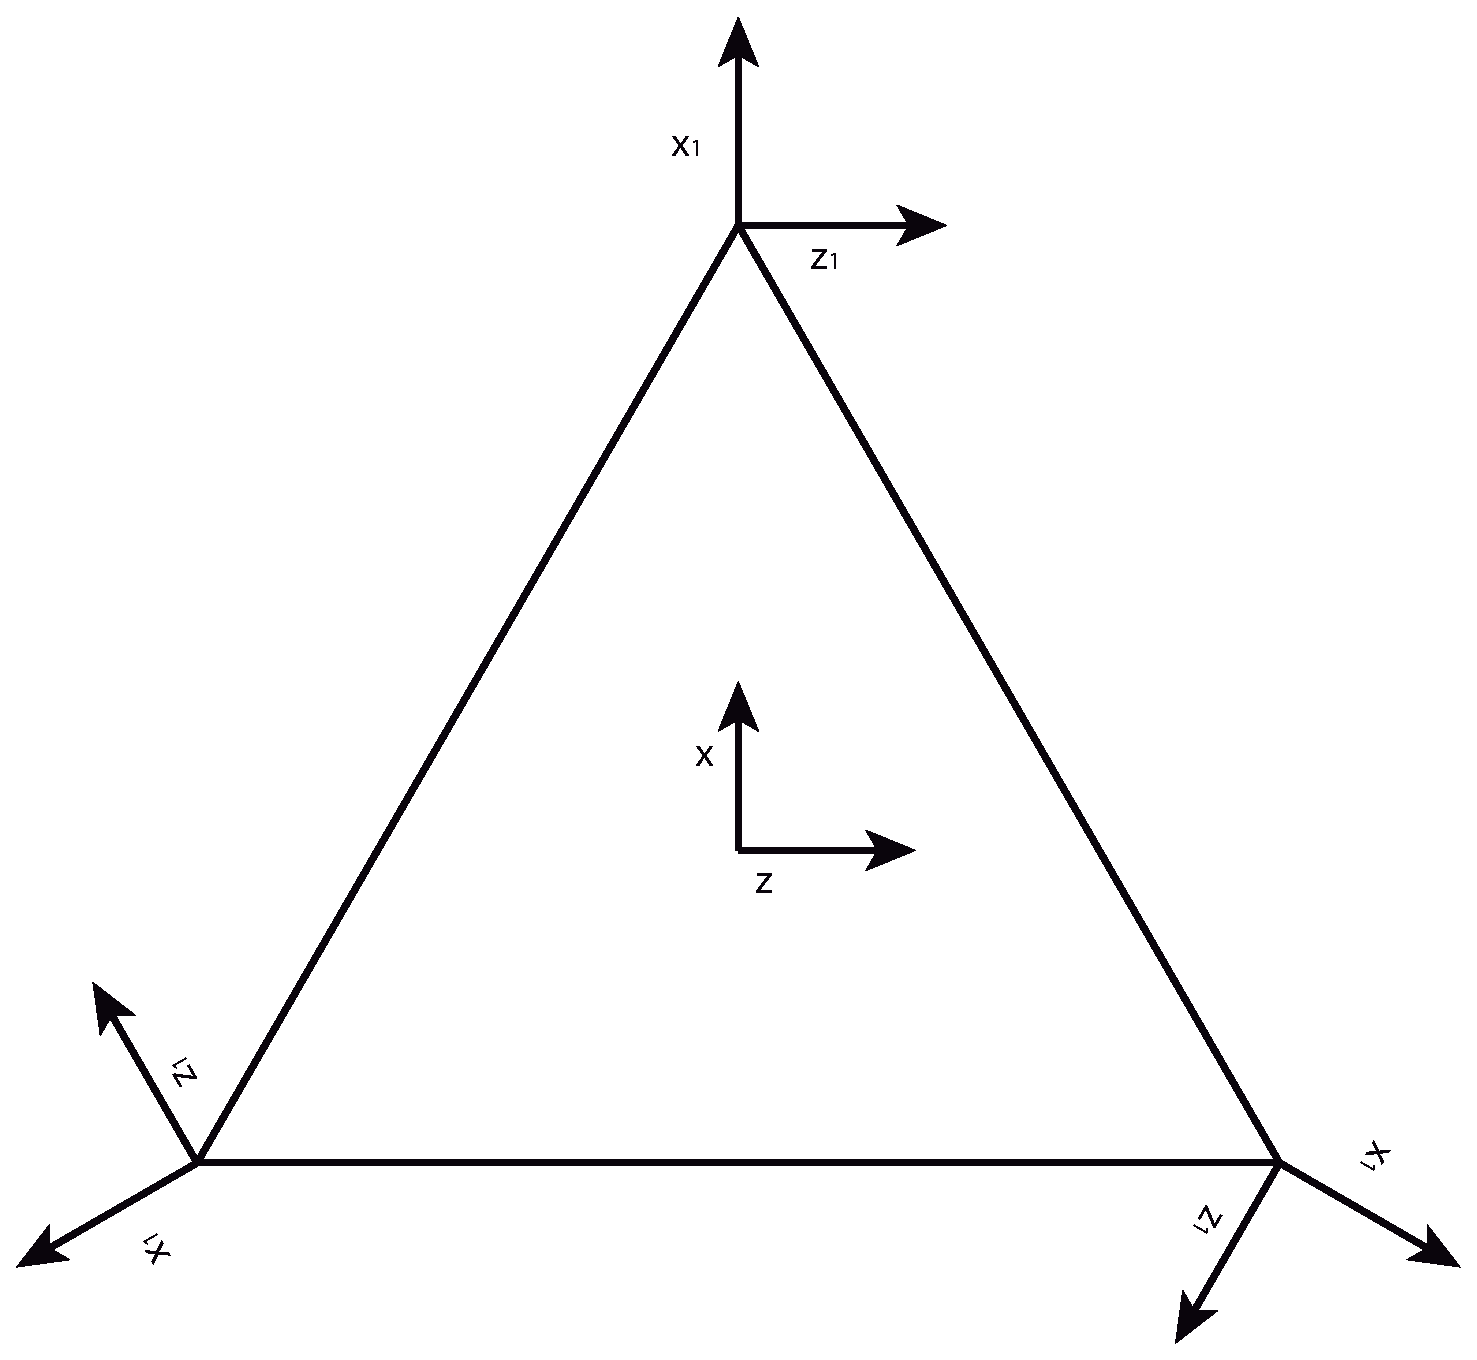
\includegraphics[width=7cm]{./sketch/canvi_base}
\end{figure}

$$\{x_1,y_1,z_1\}=\{x_0+L2-L1,y_0,z_0\}$$
$$\{x_2,y_2,z_2\}=\{z_0sin(60)-x_0cos(60)+L2-L1,y_0,-z_0cos(60)-x_0sin(60)\}$$
$$\{x_3,y_3,z_3\}=\{-z_0sin(60)-x_0cos(60)+L2-L1,y_0,-z_0cos(60)+x_0sin(60)\}$$

\subsubsection{Càlcul d'un angle}

El motor només pot moure el final del braç en un cercle, gràcies a això es poden deduir dues formules:$$x^2+y^2=a^2 \quad \textrm{i} \quad z=0$$

\begin{figure}[h!]
\centering
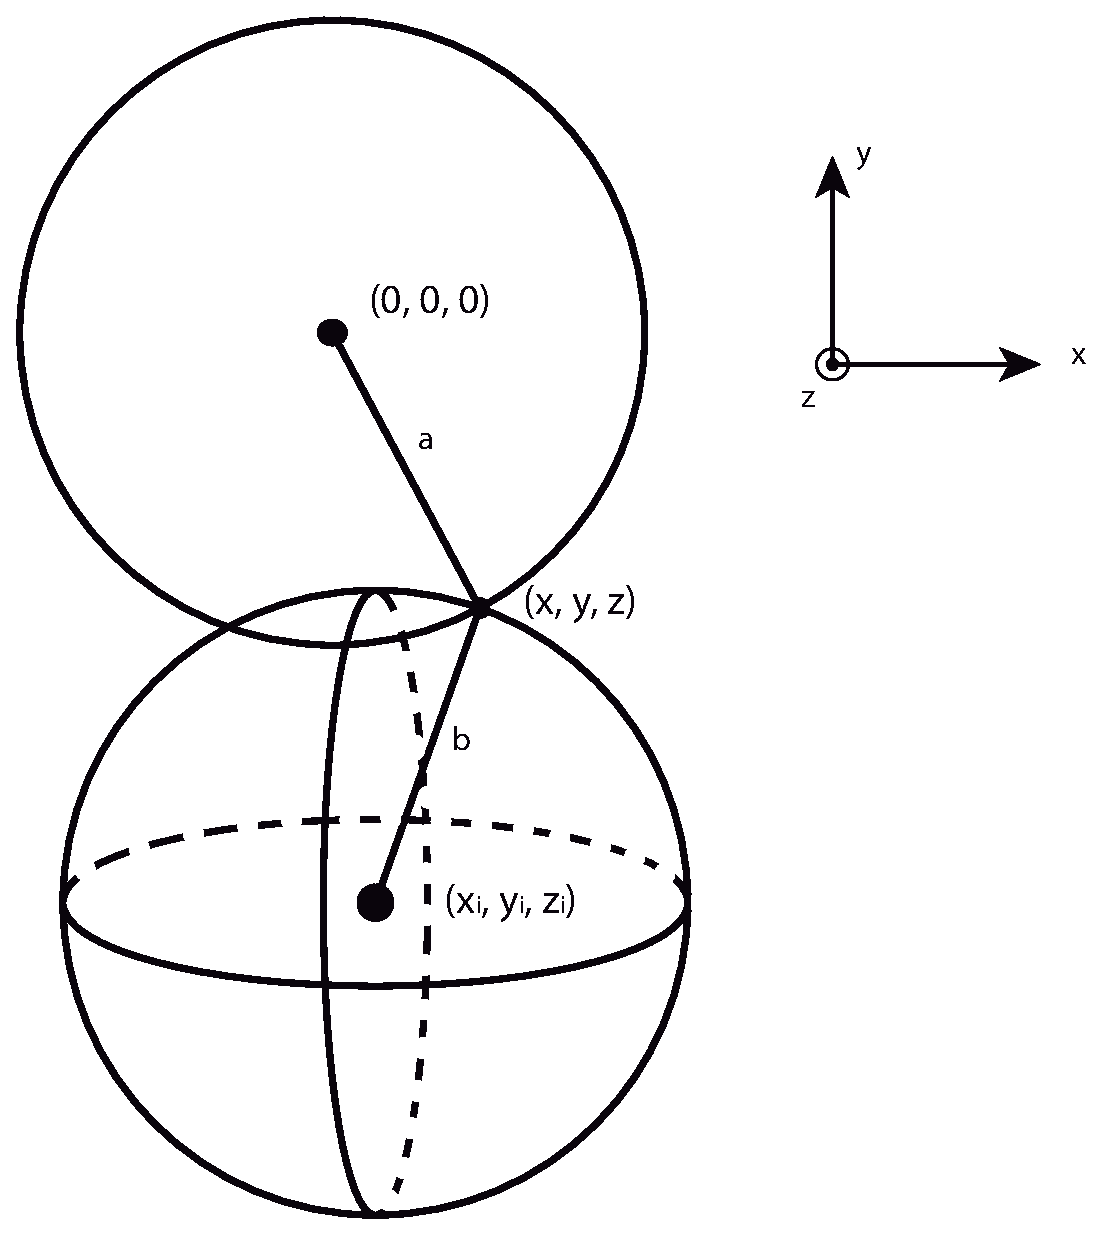
\includegraphics[width=8cm]{./sketch/calcul_angle}
\end{figure}

També es pot veure que, com ha d'estar connectat a la plataforma amb una distancia $b$ mitjançant l'avantbraç, s'ha de complir la formula: \[(x-x_i)^2+(y-y_i)^2+(z-z_i)^2=b^2\]
Ara només cal resoldre el sistema d'equacions.

\[x^2 - 2xx_i + x_i^2 + y^2 - 2yy_i + y_i^2 + z_i^2 = b^2\]
\[-2xx_i - 2yy_i = \underbrace{b^2 - a^2 - x_i^2 - y_i^2 - z_i^2}_{n}\]
\[-2x_i\sqrt{a^2-y^2}=n+2yy_i\]
\[4a^2x_i^2-4y^2x_i^2=n^2+4yy_in+4y^2y_i^2\]
\[y^2(x_i^2+y_i^2)+y(y_in)+(\frac{n^2}{4}-a^2x_i^2)=0\]
\[y=\frac{-y_i\pm\sqrt{y_i^2n^2-4(x_i^2+y_i^2)(\frac{n^2}{4}-a^2x_i^2)}}{2(x_i^2+y_i^2)}\]
\[x=\pm\sqrt{a^2-y^2}\]
\[\textrm{Finalment, }\theta=atan(\frac{y}{x})\]

\subsection{Comprovació dels càlculs}

Per poder provar les nostres funcions sense trencar el robot, es va decidir fer una simulació en del Robot en Unity. La simulació és molt simple, Unity s'encarrega de dibuixar un esquema 3D del robot utilitzant línies a partir de la posició desitjada de la plataforma i els angles del robot calculats amb la funció trobada.

\begin{figure}[h!]
\centering
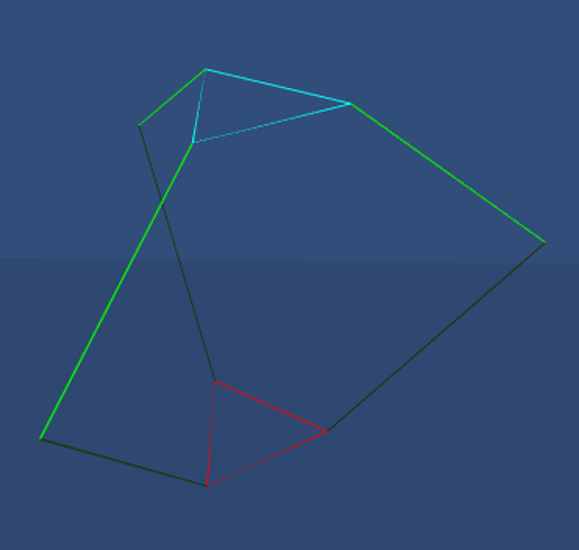
\includegraphics[width=7cm]{./images/simulacioRobot}
\end{figure}

Aquesta aplicació també es va usar per determinar quin símbol s'ha de posar abans de les dos arrels. Per la primera arrel es va determinar que havia de anar acompanyada d'un signe negatiu només quan \(x_i\) és negatiu. La segona arrel només ha de ser negativa a partir de quan el ha d'estar completament cap a dalt. La condició exacta es: \(b^2-(y_i+a)^2<x_i^2+z_i^2\) 

\newpage
\subsection{Rang de treball}

Per calcular el rang de treball s'ha utilitzat la fórmula de l'apartat anterior i buscant una gran quantitat de punts, d'aquests els que donaven un resultat possible s'han agafat com a vàlids i els altres s'han descartat. Tot seguit s'han passat els punts a Matlab\textsuperscript{\textregistered} i s'ha generat la següent superfície.

\begin{figure}[h!]
\centering
\begin{minipage}{7cm}
\centering
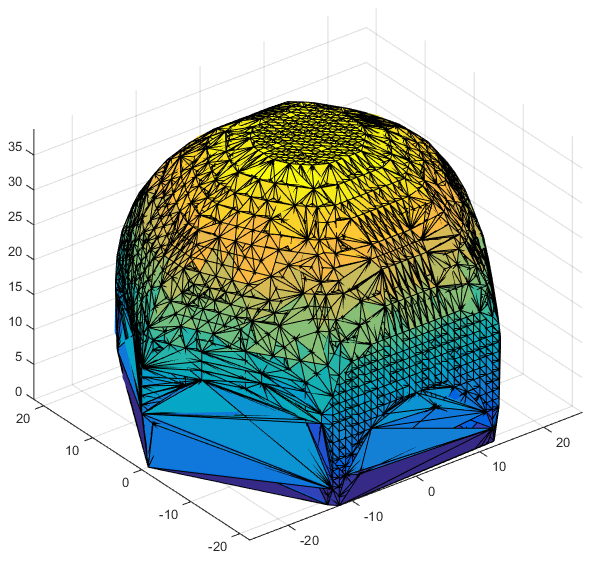
\includegraphics[width=7cm]{./images/rangTreball}
\end{minipage}
\\
\hfill
\begin{minipage}{7cm}
\centering
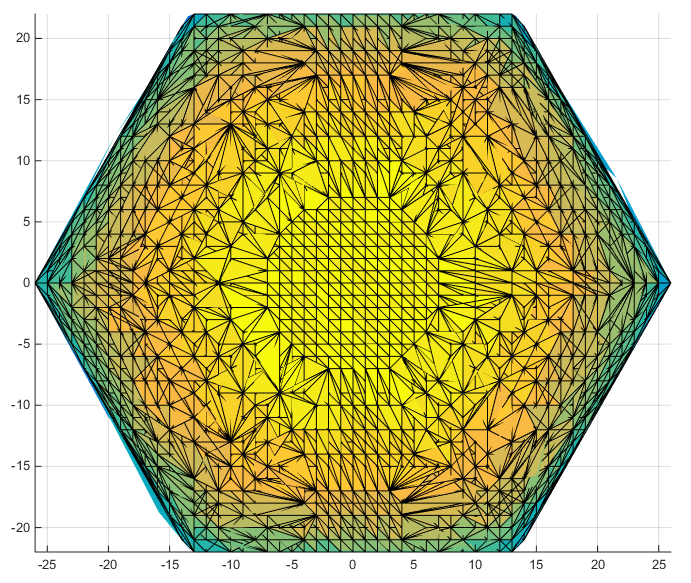
\includegraphics[width=7cm]{./images/rangTreball2}
\end{minipage}
\hfill
\begin{minipage}{7cm}
\centering
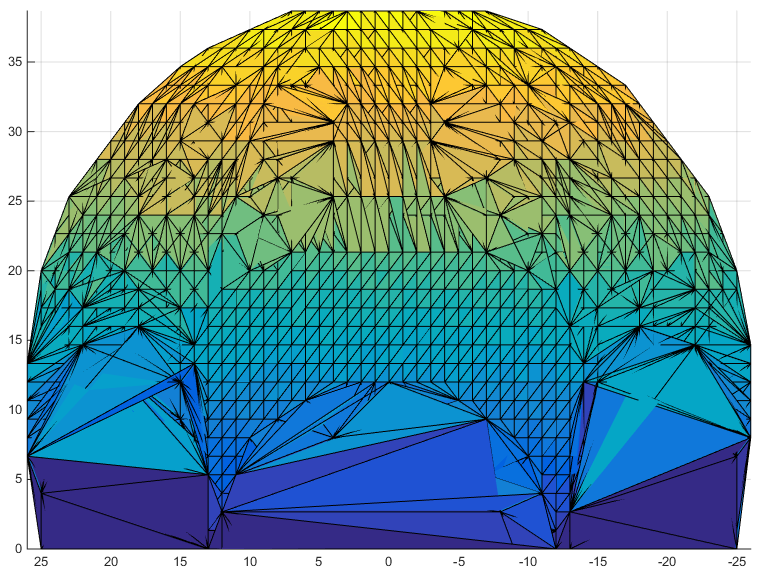
\includegraphics[width=7cm]{./images/rangTreball3}
\end{minipage}
\hfill
\end{figure}

Aquesta superfície està calculada amb tots els punts possibles teòrics però el robot te moltes limitacions mecàniques que no es tenen en compte en aquest càlcul. Per exemple els paral·lelograms dels avantbraços no poden tenir un angle qualsevol, ja que les barres de metall xoquen contra les plaques de fusta del braç si l'angle es molt petit.

\clearpage
\subsection{Implementació en Matlab}

La implementació de Matlab té tres parts, dues per al càlcul dels angles de treball i la tercera per poder calcular el rang de treball del robot.

\subsubsection{Càlcul d'un angle}
\lstinputlisting[language=Matlab]{../Matlab/singleAngle.m}

\newpage
\subsubsection{Càlcul de tots els angles}
\lstinputlisting[language=Matlab]{../Matlab/setAngles.m}

\newpage
\subsubsection{Càlcul del rang de treball}
\lstinputlisting[language=Matlab]{../Matlab/calcWorkspace.m}


\end{document}